\section{Flexible OS approaches}
\label{sec:FlexibleOSes}
The problem of overcoming disadvantages and potentially combining advantages of microkernel-based operating systems and unikernels has been addressed before. For unikernels disadvantages were a lack of isolation among components and the necessity to adapt to the component the library OS provides. Microkernels on the other hand provide strong isolation but only at the cost of significant overhead for IPC calls and again the necessity to adapt the existing code not to provided components but to communication primitives provided by the kernel. To avoid unnecessary overhead, programmers may also need to refactor the general structure of their code to minimize inter process communication. \\

One example approach is CubicleOS~\cite{sartakov2021cubicleos}. It provides three main, new abstractions to overcome the problems of the isolation vs. overhead trade-off. Those abstractions are 
\begin{enumerate}
    \item \emph{cublicles} used to define memory-isolated processes (components)
    \item \emph{windows} used to define temporary memory sharing among trusted components, and
    \item \emph{cross-cubicle calls} used to implement control flow integrity among \emph{cubicles}
\end{enumerate}
Memory isolation is implemented using Intel's Memory Protection Keys (MPK)\cite{intel64and}. A mechanism implemented in the ISA that manages access rights to virtual page tables based on keys assigned to processes. The current implementation of CubicleOS is based on the Unikraft library OS\cite{kuenzer2021unikraft}. The programmer has to specify the components that should become \emph{cubicles}. During the build process, function call among \emph{cubicles} are identified. To enforce isolation the build system of CubicleOS generates enveloping functions for those calls. These enveloping functions 
called \emph{cross-cubicle calls} implement the context switch between \emph{cubicles} at runtime. Applications using CubicleOS can run on standard Linux. To enforce memory isolation, CubicleOS comes with two runtime components one loading the components with according memory rights, one managing memory access rights. \\

The main adaptations the programmer is required to make are a) using Unikraft components b) defining the \emph{cubicles} and c) defining exceptions from the memory isolation. Exceptions are needed to improve performance and lower the overhead of context switches, when isolation is not desired. Those exception cases are either whole \emph{cubicles} or just data structures shared for particular calls among components. \emph{Cubicles} that are used frequently and are trusted can be declared 'shared' meaning  that there will be no context switches upon calls to any of their functions or usage of static constants. Data structures can be shared using CubicleOSs API for \emph{window}s, which enables the programmer to specify memory locations and sizes and the coded sections for which they should be shared. An example of this API is shown in Figure~\ref{fig:CubicleAPI}, adapted from the original publication.

\begin{figure}[H]
    %\centering
    \begin{subfigure}[b]{0.45\textwidth}
         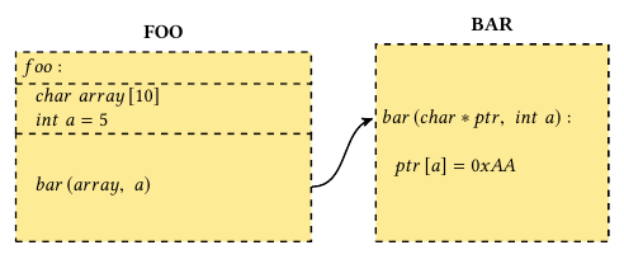
\includegraphics[width=\textwidth]{figures/cubicle_example_original.png}
         \caption{Original code of application FOO calling library BAR}
         \label{cubicleOriginal}
     \end{subfigure}
     \hfill
     \begin{subfigure}[b]{0.45\textwidth}
         %\centering
         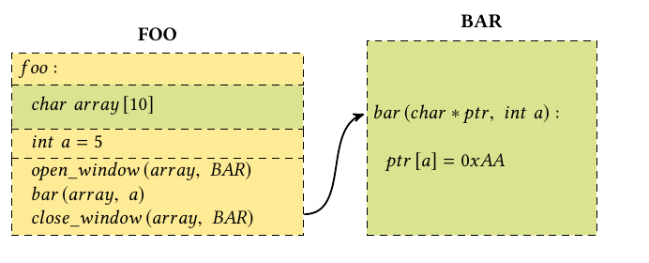
\includegraphics[width=\textwidth]{figures/cubicle_example_windows.png}
         \caption{Annotated code using Cubicles \textit{windows} to share memory after compilation}
         \label{cubicleWindow}
     \end{subfigure}
    \caption{To use Cubicle the developer basically needs to surround calls to other components, in this case BAR with \textit{windows}. Cubicle will derive isolated components and their (legitimate) interaction}
    \label{fig:CubicleAPI}
    \end{figure}

The aim of FlexOS~\cite{lefeuvre2021flexos} is to provide an easy way to exchange isolation primitives for existing code without (extensive) rewrites. Like CubicleOS it is based on an adapted version of the Unikraft library system. The two main primitives the FlexOS API provides are \emph{abstract gates} and \emph{abstract shared data}. In order to compile code with FlexOS, the programmer must replace all function calls between components with \emph{abstract gate} definitions and all shared memory areas with \emph{abstract shared data} definitions. These adjustments have also been made in the adapted system libraries. In addition the FlexOS build system needs a configuration file, which defines among other things the isolation mechanism and the division of the components. During compilation, the abstract definitions are replaced by concrete mechanisms of the target memory isolation techniques, which are MPK, Software Guard Extensions (Intel SGX) and Extended Page Tables \cite{intel64and}. \\

In comparison to our approach, FlexOS and CubileOS solve a very similar problem with very similar constraints for the programmer. She has to define components and their communication explicitly and the adaptation to a concrete architecture is only possible through compilation, because she has to select from suitable system calls and libraries in the input already. In contrary to those systems, we do not provide an API to explicitly allow data sharing via references. It is possible to use reference sharing in Ohuas input programs, as only explicit reference passing is excluded. However Ohua will tread arguments passed by reference the same way as arguments passed by value. So if the resulting program is functional and if pass-by-reference is any more efficient than pass-by-value depends on the target architecture. Which also means we could not effectively use FlexOS or CubileOS as backend integrations.


\section{Compiling to State Local Programs}

Of course, many of the problems and approaches that emerged in the implementation are not new. Denationalization as a concept for mapping higher-order functions to serializable data types was first presented in the work of Reynolds~\cite{reynolds1972definitional}. Building on that concept, as well as Danvy~\cite{danvy2008defunctionalized} discussed how defunctionalization and refactoring to continuation passing style (CPS) can be used to transform programs with structural operational semantics (including interruptions and errors) to reduction semantics. The author integrates their results with previous work yielding the transformation based equivalence graph shown in Figure~\ref{fig:transformationsDanvy}. Given those results we can explore and maybe better describe in future what our transformations should be, for example it would also be conceivable to defining stateful objects as abstract machines within the DFG. In a subsequent work Danvy and Millikin~\cite{DANVY2009534} present \emph{Refunctionalization} as the left inverse of Defunctionalization. This transformation can be applied as an intermediate step, if programs are not directly amenable to defunctionalization. As the authors describe it ``A program can fail to be in the image of defunctionalization if there are multiple points of consumption for elements of a data type or if the single point of consumption is not in a separate function´´. Considering the initial structure of the \rust{poll} function, the transformation described by Danvy and Millikin might also be necessary to formalize the findings in this work.

\begin{figure}[H]
\centering
   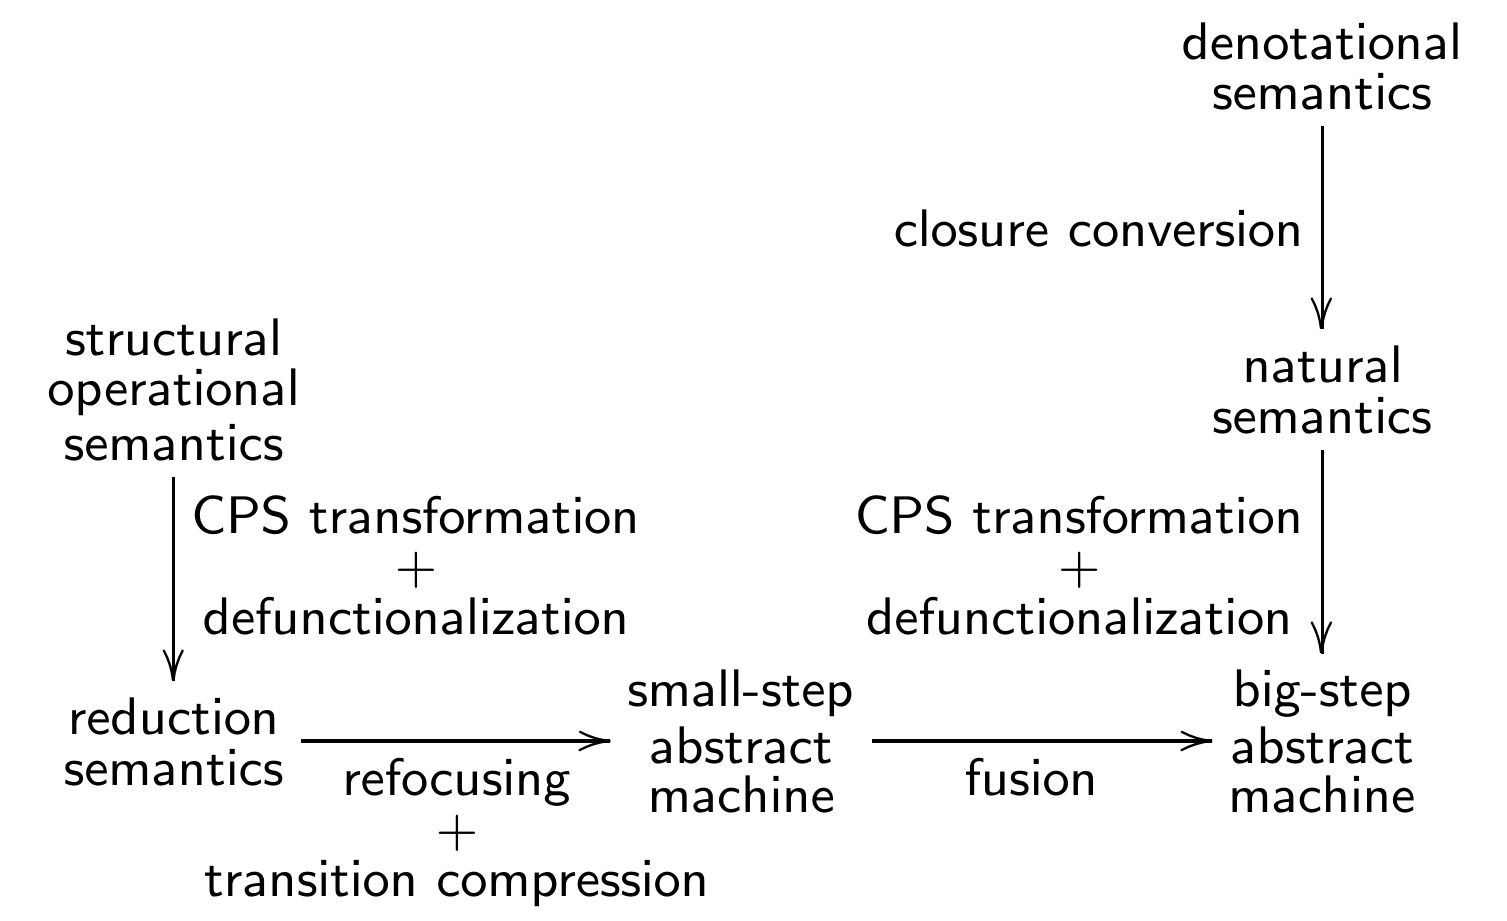
\includegraphics[width=0.6\textwidth]{figures/transformations_danvy.png}
\caption{Graph representing the inter-derivability relation of different abstract models for computation, taken from Danvy~\cite{danvy2008defunctionalized}}
\label{fig:transformationsDanvy}
\end{figure}

The paper \emph{Automatically Restructuring Programs for the Web}~\cite{graunke2001automatically} also applies refactoring to CPS followed by defunctionalization. They target the transformation of local, interactive programs to web CGI programs. As with the \stack{.poll} function in our case, the control flow in the source program is continuous in or above the stack frame of the server functions, while the target setting requires explicit handling of both the control flow and the stack state upon leaving an reentering the server function. The paper presents a 
 prototypical implemented automated transformations, to turn a local interactive program into a CGI program. Interestingly in Scheme, the implementation language used, continuations are first-class members and could be stored and reapplied to stack directly assigning each a specific URL, such that the client request can directly address the continuation. Problem was that this was a) language specific and b) had lots of overhead for a distributed garbage collection of stored continuations. So the solution was to embed the control flow into the data flow using defuncionalized representations of entry points. To handle stateful objects, i.e. in general any variable that is reassigned in different invocations of the server, they use the Scheme concept of \code{boxes}. This approach is very similar to what has been done in this work, e.g. by making part of the state of the interface. They must be defined globally, are loaded on each call (from memory or a cookie) and allow all sub-functions of the original server function to access the stateful variable. Considering the server-client setting, the authors also comment on security considerations. The transformations made de facto lead to control flow being integrated into the data flow and, in the case of a web application, can be changed by a malicious user. Even if we aim at a different application scenario, we should evaluate which parts of the control flow actually need to be integrated into the data flow. The security measures proposed by the authors mainly concern the cryptographic protection of the communication and are in this respect possibly a question for further architecture integrations in Ohua. \\

The problem of managing stack based data in event-driven and cooperative programming has  also been addressed in \cite{adya2002cooperative}. Ohua doesn't explicitly aim at event-driven programs. However we have seen that the principle problem of shifting from automatic stack management to a control-flow "re-entering", necessitates to either store and retrieve the execution state explicitly or send parts of it along the data flow, or even passing respectively. The authors discuss necessary refactoring steps to transform single-threaded programs to either a multi-threaded, preemptively scheduled  or even-driven versions. Regardless of the final form, they described the necessity of ``Stack Ripping´´, i.e. manually handling the information formerly based on a single function stack. While they use a different vocabulary, the core points of the transformations are actually the same as in the works cited before, facing four main requirements for the  implementation resulting from ``Stack Ripping´´
\begin{enumerate}
    \item lifting closures: Parts of functions interleaved with I/O actions or calls to other components need to become language-level functions.
    \item function scope: As more than one function now represent what was one function before the original environment of the code in each sub-function must be manually preserved
    \item automatic variables: variables that where allocated on the stack, but need to survive multiple function calls now, must be allocated on the heap
    \item control structures: Structures like loops or branches lead to additional entry point functions
\end{enumerate}

 Further they describe how in Windows, \code{fibers} and \code{threads} are used to implement interactions between applications using manual or automatic stack management respectively. The identified requirements are very much in line with the necessary refactorings we identified. 


\section{(Automatic) Memory Isolation}
\label{sec:MemoryIsolation}
Besides virtualization and the direct implementation of microkernel-based systems, there are also other approaches to address the security problem of the lack of isolation. One such system is \emph{Hardware-Assisted Kernel Compartmentalization}(HAKC)\cite{mckee2022preventing}. The authors exemplify the problem for Loadable Kernel Modules (LKM), which are themselves not a part of the Linux kernel but loaded and executed in 
kernel space. With many of them providing audio and media processing and drivers, they are a notorious entry point for system compromise exploiting local bugs. In particular they describe an example CVE, where the exploit neither violates memory safety nor control flow integrity and could hence only be prevented by compartmentalization of the modules involved and a defined interfacing to the kernel. HAKC provides an API to define components and a hardware-based runtime system to enforce in-kernel isolation of the defined components. This API allows the programmer to assign compilation units, files or smaller fractions of code into logical units \emph{Cliques} and \emph{Compartments} and define directional memory access and control-flow policies among them. So the actual compartments and access rules are entirely made by the programmer and HAKC itself, does not check or optimize isolation policies. The hardware mechanisms used to enforce the derived policies are called \emph{pointer authentication} (PAC), introduced in ARMv8.3 and \emph{memory tagging extension}(MET), introduced in ARMv8.5-A. The basic principle of TAC is to have pointers cryptographically signed by their legitimate owner, store the signature in the pointer and only allow access based on pointer authentication. MET allows to assign memory regions to different tags and use those groupings to manage access policies. Measured with  different microbenchmarks the overhead for HAKC policy enforcement on the \code{ipv6.ko} LKM imposed a runtime overhead of 1.6\% to 24\% for individual benchmarks.\\

To overcome the difficulty of manually identifying dependencies among components \emph{FlexC}\cite{mckee2022novel} was later presented as an approach to automatically generate the compartmentalization policies that HAKC requires as interface definition among components. The authors argue that in particular in larger system hand-written annotations are error prone and might also lead to inefficient choices. Like HAKC itself, FlexC uses static information from the input code, to generate a data access graph from the input program. To account for indirect data access via pointers the analysis conservatively overestimates potential dependencies. Dynamic data i.e. test runs of the input code can additionally be provided to weighten the data dependencies by frequency of access and size of data. To start the derivation FlexC automatically assigns compilation units (in C usually one ore more files) as smallest entity of isolation. By defining the target number of compartments, the programmer can initialize a greedy fusion of nodes after the initial graph was build, generating a coarser compartmentalization. It is also possible to manipulate the graph using a GUI for FlexC. The output of FlexC is then directly integrated to the compilation process using HAKC. \\

Since most hardware-related, system-level code is still written in C and C++, the approach of \emph{Spons \& Shields}\cite{SponsAndShields} directly builds on these languages. However  they focus rather on a scenario commonly encountered in cloud deployments, namely the usage of \emph{Trusted Execution Environments} based on Intel SGX TEEs. TEEs are increasingly popular for secure cloud deployments and while they where initially used to encapsulate only specific critical user applications, they are now used to move whole OSes into a single secure environment e.g. into an Intel SXG enclave. The identified problem is, again that this creates large code spaces without internal access restrictions and possibly including insecure, third party libraries, which contradicts the defense in depth approach. The next problem the authors notice is that compartmentalization is often enforced along processes. But it is hard to redesign an application to encapsulate different concerns and security levels into different processes. Also the trust model of TEEs does not include the host, while process isolation techniques are based on the primitives the host OS and hardware (MMU) provide. The Spons\& Shields framework (SSF) described in the paper consists of an API to manage the two core abstractions \emph{Spons}, which encapsulate units of execution, e.g. POSIX processes or libraries and \emph{Shields} which define hierarchical memory access regions. The programmer needs to introduce \emph{Spons} and \emph{Shields} according to her requirements in the code and link against the \code{musl} standard C library. During compilation the framework will insert TEE primitives to enable the SSF runtime to enforce memory boundaries between the Spons. To benchmark their technique they used the scenario of a web application consisting of an NGNIX server, a PostreSQL data base (with medical data), an SSL library for crypto and a business logic application in PHP. They compared request latency for a single TEE vs. multi-TEE compartments vs. Shielded deployment and found that shields increase latency by about 1.7 times using Shields while multiple TEEs increased latency about 4.4 times compared to the single TEE version.\\

 \emph{PKRU-Safe}\cite{kirth2022pkru} is an approach with a slightly different target. Instead of vertical compartmentalization it intends to enforce a separation between memory safe and memory unsafe code in Rust applications. The identified problem is that safe languages in this case Rust are already available and it should be possible to interact with unsafe language components without risking memory corruption. So the whole point is to enforce hierarchic/semi-permeable memory isolation between Rust code and unsafe languages. The concept is to have the developer explicitly define the interface between trusted and untrusted parts of the code. This is done via annotations in the projects build file and the untrusted libraries. With per library annotations the adaptation overhead is significantly smaller than in annotating single functions or data access. To analyse the code and track heap allocations PKRU-Safe uses custom plugins to rustc and LLVM tooling. To identify the usage sites of heap allocated data the input program is run with provided profiling input to dynamically identify when the untrusted component accesses data allocated by the trusted component. The gathered access data are used to categorize data allocation into unsafe and safe memory, in particular data that is used by unsafe code is considered belonging to the unsafe code. At runtime this distinction is used to enforce the policy that unsafe code can never access safe memory. To move such data into the untrusted component entirely and to handle the two memory pools at run time the \rust{liballoc} to augment it by dedicated primitives for unsafe memory allocation. The authors describe this runtime behavior as \emph{compartment-aware} heap allocation. By keeping heap section of safe and unsafe memory objects distinct, PKRU-Safe can implement the policies using MPK protection for the trusted heap section. Notably this policy only applies to data on the heap. Stack data is assumed to be protected by other mechanisms. They apply the concept to Servo, a layout-engine written in Rust and tested the performance overhead with different benchmark suites (Dromaeo, Kraken, Octane and JetStream2). They found the altered allocation mechanism to cause an average runtime overhead of 6\% above baseline. The overhead imposed by context switches  involving MPK depended on the concrete benchmark with an average of 11\% and a maximum of about 30\%. \\

Contrary to the Ohua approach, these techniques are currently bound to a particular language and particular hardware mechanisms. On the one hand this enables a deeper analysis of the code, in particular if also dynamic information is considered. It can also lower the imposed overhead, because a distinction between memory sharing and memory transfer can be made. On the other hand it limits the flexibility. All of the approaches require additional programmer information to identify the target components, but also to shape the intended isolation policies. In how far data of one component is still accessible to the other is in case of Ohua, depending on the chosen architecture integration and the programmers compliance to the programming model, in case the architecture permits the usage of shared references. 
